% Generated by figures/make_figures.py -- do not edit by hand.
% Requires \usepackage{pgfplots} and \pgfplotsset{compat=1.18} in the preamble.

\begin{figure}[htbp]
\centering
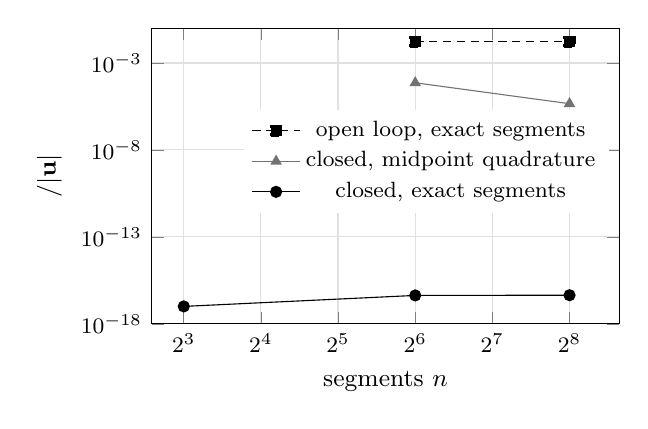
\begin{tikzpicture}
\begin{axis}[
  width=0.62\textwidth, height=0.44\textwidth,
  xlabel={segments $n$}, ylabel={$\eps/|\mathbf{u}|$},
  xmode=log, ymode=log, log basis x=2,
  xmin=6, xmax=400, ymin=1e-18, ymax=1e-1,
  grid=both, grid style={black!12},
  tick label style={font=\footnotesize}, label style={font=\small},
  legend style={font=\footnotesize, at={(0.98,0.55)}, anchor=east, draw=none},
]
\addplot[black, mark=square*, densely dashed]
  coordinates {(64,1.68e-2) (256,1.68e-2)};
\addlegendentry{open loop, exact segments}
\addplot[black!55, mark=triangle*]
  coordinates {(64,7.28e-5) (256,4.56e-6)};
\addlegendentry{closed, midpoint quadrature}
\addplot[black, mark=*]
  coordinates {(8,1e-17) (64,4.28e-17) (256,4.4e-17)};
\addlegendentry{closed, exact segments}
\end{axis}
\end{tikzpicture}
\caption{The discrete residual carries no resolution floor. With exact segment
integration the grade-3 term telescopes, so a closed filament of constant
circulation cancels to round-off at any number of segments --- detected already
at $n=8$, and unaffected by mollification. Midpoint quadrature instead leaves an
$O(h^2)$ floor which would mask a genuine closure violation of comparable size.
Removing one segment separates the closed and open cases by fifteen orders of
magnitude. The closed-exact values are at the round-off level and are plotted at
their measured magnitudes; the $n=8$ point measured exactly zero and is drawn at
the double-precision floor.}
\label{fig:closure}
\end{figure}

\begin{figure}[htbp]
\centering
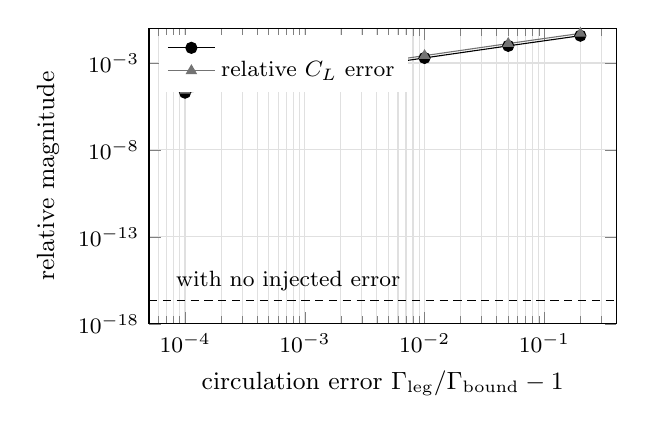
\begin{tikzpicture}
\begin{axis}[
  width=0.62\textwidth, height=0.44\textwidth,
  xlabel={circulation error $\Gamma_{\mathrm{leg}}/\Gamma_{\mathrm{bound}} - 1$},
  ylabel={relative magnitude},
  xmode=log, ymode=log, xmin=5e-5, xmax=0.4, ymin=1e-18, ymax=1e-1,
  grid=both, grid style={black!12},
  tick label style={font=\footnotesize}, label style={font=\small},
  legend style={font=\footnotesize, at={(0.02,0.98)}, anchor=north west,
                draw=none},
]
\addplot[black, mark=*]
  coordinates {(1e-4,1.96e-5) (1e-3,1.96e-4) (1e-2,1.96e-3)
               (5e-2,9.68e-3) (2e-1,3.72e-2)};
\addlegendentry{$\eps$}
\addplot[black!55, mark=triangle*]
  coordinates {(1e-4,2.66e-5) (1e-3,2.66e-4) (1e-2,2.65e-3)
               (5e-2,1.31e-2) (2e-1,5.05e-2)};
\addlegendentry{relative $C_L$ error}
\addplot[black, densely dashed, domain=5e-5:0.4, forget plot] {2.3e-17};
\node[anchor=south west, font=\footnotesize] at (axis cs:6e-5,2.3e-17)
  {$\eps$ with no injected error};
\end{axis}
\end{tikzpicture}
\caption{Detection of a circulation-conservation error in an elliptic-wing
vortex lattice. Within this perturbation family the residual is proportional to
the lift error, the ratio holding to three digits across four decades. The
dashed line is the residual of the unperturbed lattice: a $0.01\%$ circulation
error moves $C_L$ by $\num{2.7e-5}$, which no force-based check would flag, while
lifting $\eps$ twelve orders of magnitude above its clean value.}
\label{fig:detection}
\end{figure}

\begin{figure}[htbp]
\centering
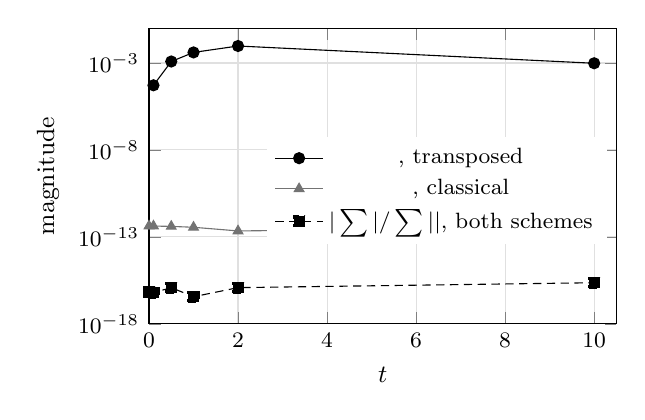
\begin{tikzpicture}
\begin{axis}[
  width=0.62\textwidth, height=0.44\textwidth,
  xlabel={$t$}, ylabel={magnitude}, ymode=log,
  xmin=0, xmax=10.5, ymin=1e-18, ymax=1e-1,
  grid=both, grid style={black!12},
  tick label style={font=\footnotesize}, label style={font=\small},
  legend style={font=\footnotesize, at={(0.98,0.45)}, anchor=east, draw=none},
]
\addplot[black, mark=*]
  coordinates {(0.1,5.22e-5) (0.5,1.22e-3) (1.0,4.06e-3) (2.0,9.50e-3)
               (10.0,9.66e-4)};
\addlegendentry{$\eps$, transposed}
\addplot[black!55, mark=triangle*]
  coordinates {(0,4.19e-13) (0.1,4.18e-13) (0.5,4.00e-13) (1.0,3.56e-13)
               (2.0,2.19e-13) (10.0,3.58e-13)};
\addlegendentry{$\eps$, classical}
\addplot[black, mark=square*, densely dashed]
  coordinates {(0,6.8e-17) (0.1,6.2e-17) (0.5,1.2e-16) (1.0,3.6e-17)
               (2.0,1.2e-16) (10.0,2.3e-16)};
\addlegendentry{$|\sum\balpha|/\sum|\balpha|$, both schemes}
\end{axis}
\end{tikzpicture}
\caption{An emergent violation that no local check can see. An elliptical vortex
ring of 200 particles is advanced under the two standard stretching
discretisations from a common machine-zero start. A material line element obeys
$\dd(\dd\boldsymbol{\ell})/\dd t = (\dd\boldsymbol{\ell}\cdot\nabla)\bu$, which is
the classical scheme, so a filament-derived particle set retains its structure
under it. The transposed scheme drifts ten orders of magnitude within a tenth of
a time unit. Throughout, the conservation check a practitioner would normally
rely on sits at machine precision for both schemes and detects nothing.}
\label{fig:vpm}
\end{figure}
